\section{Magnet Grade Selection and Rotor Temperature}\label{sec:grades}
\begin{figure*}[!t]
\centering
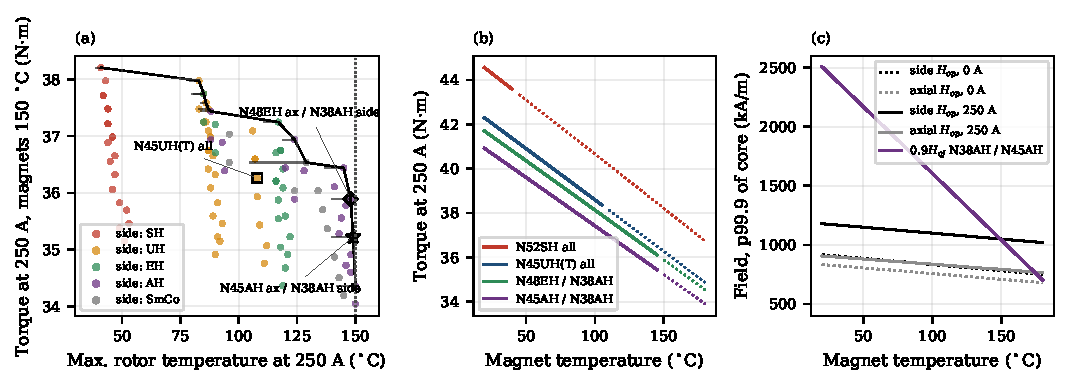
\includegraphics[width=\textwidth]{grades.pdf}
\caption{Magnet grade selection, 40Cr-backed v4b rotor, ideal materials. (a) All 100 axial/side grade pairs: torque at \SI{250}{A} with \SI{150}{\celsius} magnets against the highest magnet temperature that passes the knee criterion at \SI{250}{A}. The black line is the Pareto front; the whiskers reach the 95\,\% (5th-percentile) temperature from Monte Carlo. (b) Torque against magnet temperature at \SI{250}{A}; dotted where the pair would be partially demagnetised. (c) Recommended pair: 99.9th-percentile reverse field in the side and axial pieces against the knee of N38AH/N45AH.}
\label{fig:grades}
\end{figure*}

The rotor is now fixed as the v4b Halbach array on a \SI{1}{mm} quenched-and-tempered 40Cr back ring. 4140 or 4340 steel can be used for the ring instead. All three are medium-carbon Cr(--Mo/Ni) alloy steels with similar saturation. The ring is modelled with an estimated Q\&T 40Cr $B$--$H$ curve, and 2-D runs showed the ring material changes torque by less than \SI{1}{\percent}. The stator winding is limited to \SI{150}{\celsius}. A magnet set that tolerates \SI{150}{\celsius} at full current therefore removes the rotor as a separate thermal limit. This section asks which magnet grade, or pair of grades, gives the most torque under that constraint.

\subsection{N45UH(T) on the 40Cr ring}
Direct 3-D solves with N45UH-class magnets ($B_r=\SI{1.35}{T}$ at \SI{20}{\celsius}, $-\SI{0.12}{\percent/K}$, from the Arnold GB45UH datasheet) give \SI{42.2}{\Nm} at \SI{250}{A} with \SI{20}{\celsius} magnets, and \SI{39.6}{\Nm} at \SI{80}{\celsius}. The catalogue rating of \SI{180}{\celsius} for this class applies to a magnet in its own field at a moderate permeance coefficient. In the Halbach array the side (tangentially magnetised) pieces also carry the reverse field of their neighbours and of the stator. The 99.9th percentile of that field in their core is \SI{0.97}{MA/m} at no load and \SI{1.23}{MA/m} at \SI{250}{A}. With the knee criterion $H_{op}\le0.9H_{cJ}(T)$, N45UH(T) is limited to about \SI{108}{\celsius} at \SI{250}{A}.

\begin{figure*}[!t]
\centering
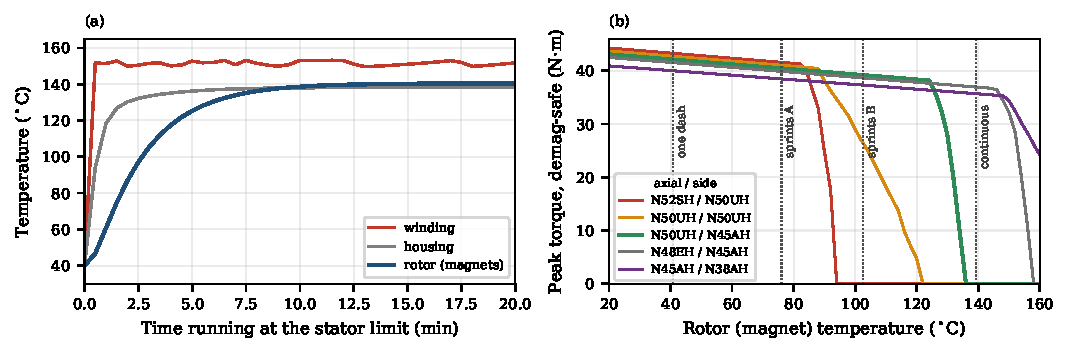
\includegraphics[width=\textwidth]{rotor_thermal.pdf}
\caption{(a) Winding, housing and rotor temperature when the motor runs continuously at its \SI{150}{\celsius} winding limit, starting from \SI{40}{\celsius}. (b) Peak torque available without demagnetisation against rotor temperature for candidate pairs (axial/side), with current limited where needed to stay below the knee (ideal materials). Dotted lines mark the rotor temperatures of \cref{tab:rotorT}: one dash; repeated sprints resting to \SI{70}{\celsius} (A) and to \SI{100}{\celsius} (B); continuous running at the limit.}
\label{fig:rotorT}
\end{figure*}

\subsection{Surrogate model and Monte Carlo search}
The magnets are linear ($\mu_r=1.05$), so the field at any point in them depends on three inputs: the remanence of the axial pieces $B_{r,a}$, the remanence of the side pieces $B_{r,t}$ and the current. Nine 3-D solves were run on one mesh, spanning $B_{r,a},B_{r,t}\in[1.0,1.3]$\,T and $I\in\{0,150,250\}$\,A. At each of \num{2e5} fixed sample points in the magnets, $\bm{M}\cdot\bm{B}$ was fitted to $\{1,B_{r,a},B_{r,t},I,I^2\}$. Torque at \SI{250}{A} was fitted bilinearly in the two remanences. The surrogate was checked against FEA it was not fitted to:
\begin{itemize}
\item a held-out solve at $(1.18,1.12)$\,T, \SI{250}{A}: the field percentiles are within \SI{0.6}{\percent} and torque within \SI{0.2}{\percent};
\item the six independent N45UH(T) solves at \SIlist{1.35;1.25}{T}, outside the fitted range: the field percentiles are within \SI{0.7}{\percent} and torque within \SI{0.3}{\percent}.
\end{itemize}
Each evaluation then costs milliseconds instead of 20 minutes, which makes an exhaustive search with Monte Carlo tolerance analysis possible.

\begin{table}[!t]
\caption{Magnet grade catalogue (typical $B_r$, minimum $H_{cJ}$ at \SI{20}{\celsius})}\label{tab:catalogue}
\centering\scriptsize\setlength{\tabcolsep}{4pt}
\begin{tabular}{@{}lccccc@{}}
\toprule
Grade & $B_r$ & $H_{cJ}$ & $\alpha_{B_r}$ & $\beta_{H_{cJ}}$ & $H_k/H_{cJ}$\\
 & (T) & (kA/m) & (\si{\percent/K}) & (\si{\percent/K}) & \\
\midrule
N52SH & 1.43 & 1592 & $-0.12$ & $-0.55$ & 0.90\\
N50SH & 1.40 & 1592 & $-0.12$ & $-0.55$ & 0.90\\
N50UH $^\dagger$ & 1.40 & 1990 & $-0.12$ & $-0.50$ & 0.90\\
N48UH & 1.37 & 1990 & $-0.12$ & $-0.52$ & 0.90\\
N45UH(T) $^\dagger$ & 1.35 & 2149 & $-0.12$ & $-0.47$ & 0.90\\
N48EH $^\dagger$ & 1.37 & 2388 & $-0.12$ & $-0.48$ & 0.90\\
N42EH & 1.30 & 2388 & $-0.12$ & $-0.50$ & 0.90\\
N45AH $^\dagger$ & 1.33 & 2786 & $-0.12$ & $-0.45$ & 0.90\\
N38AH & 1.24 & 2786 & $-0.11$ & $-0.45$ & 0.90\\
Sm$_2$Co$_{17}$ 32H & 1.13 & 1990 & $-0.035$ & $-0.20$ & 0.70\\
\bottomrule
\multicolumn{6}{@{}l}{$^\dagger$Usually grain-boundary-diffused (GBD).}
\end{tabular}
\end{table}

\Cref{tab:catalogue} lists the ten grades considered. The values are typical datasheet figures and must be confirmed with the chosen supplier. All 100 axial/side pairs were evaluated.

\textbf{Demagnetisation criterion.} The 99.9th percentile of $H_{op}$ in the core of each piece type, excluding \SI{0.2}{mm} at the top and bottom faces, must stay below the knee $H_k=k\,H_{cJ}(T)$, with $H_{cJ}(T)=H_{cJ,20}[1+\beta(T-20)]$.

\textbf{Monte Carlo.} For each pair, 1500 samples were drawn, with each piece type taken from one magnet lot:
\begin{itemize}
\item $B_r$ normally distributed, $\sigma=\SI{0.75}{\percent}$;
\item $\alpha$ within \SI{\pm0.01}{\percent/K};
\item $H_{cJ}$ between \SI{0}{\percent} and \SI{8}{\percent} above the guaranteed minimum;
\item $\beta$ within \SI{\pm0.04}{\percent/K};
\item squareness $k$ within its typical band;
\item a \SI{3}{\percent} (1$\sigma$) error on the computed field.
\end{itemize}
For each pair this gives the nominal maximum magnet temperature at \SI{250}{A}, its 5th percentile (the temperature met by \SI{95}{\percent} of builds), and the probability of passing at \SI{150}{\celsius}.



\begin{table}[!t]
\caption{Magnet grade pairs on the 40Cr-backed v4b rotor (ideal materials, \SI{250}{A})}\label{tab:grades}
\centering\footnotesize
\begin{tabular}{@{}llcccc@{}}
\toprule
Axial & Side & \multicolumn{2}{c}{$T_\mathrm{mag,max}$ (\si{\celsius})} & \multicolumn{2}{c}{Torque (\Nm)}\\
\cmidrule(lr){3-4}\cmidrule(l){5-6}
pieces & pieces & nominal & 95\,\% & \SI{150}{\celsius} & \SI{20}{\celsius}\\
\midrule
N52SH & N52SH & 41 & 39 & 38.2 & 44.6\\
N50UH & N50UH & 87 & 83 & 37.5 & 43.7\\
N45UH(T) & N45UH(T) & 108 & 104 & 36.3 & 42.3\\
N50UH & N45AH & 124 & 119 & 36.9 & 43.1\\
\textbf{N48EH} & \textbf{N45AH} & \textbf{145} & \textbf{137} & \textbf{36.4} & \textbf{42.5}\\
N45AH & N45AH & 146 & 139 & 35.8 & 41.7\\
N48EH & N38AH & 148 & 140 & 35.9 & 41.7\\
N45AH & N38AH & 149 & 140 & 35.2 & 40.9\\
Sm$_2$Co$_{17}$ & N38AH & 150 & 142 & 34.4 & 37.0\\
\bottomrule
\end{tabular}
\end{table}


\subsection{Results}
\Cref{fig:grades} and \cref{tab:grades} give the results.
\begin{itemize}
\item \textbf{SH and UH grades cannot reach \SI{150}{\celsius} in this rotor.} At \SI{250}{A}, N52SH is limited to \SI{41}{\celsius}, N50UH to \SI{87}{\celsius} and N45UH(T) to \SI{108}{\celsius}. Their extra \SIrange{2}{3}{\Nm} at temperature cannot be used.
\item \textbf{The side pieces set the limit, and a lower-$B_r$ grade helps there.} The reverse field in a side piece grows faster with its own remanence than with that of the axial pieces (\SI{+121}{kA/m} against \SI{+84}{kA/m} for \SI{+0.3}{T} at \SI{250}{A}), so N38AH side pieces reach a higher temperature than N45AH side pieces.
\item \textbf{The axial pieces carry the torque.} Swapping the remanences of the two sets ($1.3/1.0$ against $1.0/1.3$\,T) changes torque from \SI{38.1}{\Nm} to \SI{35.0}{\Nm}. High-$B_r$ magnets therefore belong in the axial pieces, provided they meet the lower field there.
\item \textbf{Best pair for a \SI{150}{\celsius} rotor: N45AH axial pieces with N38AH side pieces.} This pair holds \SI{149}{\celsius} at \SI{250}{A} nominally and \SI{140}{\celsius} for \SI{95}{\percent} of builds. It survives \SI{175}{\celsius} at no load and gives \SI{35.2}{\Nm} with \SI{150}{\celsius} magnets and \SI{40.9}{\Nm} at \SI{20}{\celsius}.
\item \textbf{N48EH axial pieces with N38AH side pieces} give \SI{1.9}{\percent} more torque, but its no-load limit is only \SI{160}{\celsius}. It is also less robust, passing \SI{150}{\celsius} at \SI{250}{A} in \SI{49}{\percent} of samples against \SI{68}{\percent} for N45AH/N38AH.
\item \textbf{No catalogue pair passes \SI{250}{A} at \SI{150}{\celsius} with \SI{95}{\percent} confidence.} With N45AH/N38AH, \SI{95}{\percent} of builds can take \SI{163}{A} at \SI{150}{\celsius}, or \SI{250}{A} up to \SI{140}{\celsius}. Rounding the inner corners of the side pieces, where the field peaks, is the remaining design lever.
\end{itemize}

A rotor held at \SI{150}{\celsius}, however, is a worst case that the next subsection shows does not occur in use.

\subsection{Rotor temperature in use}
The rotor has no copper loss. Its own losses are eddy currents in the segmented magnets and the 40Cr ring, estimated at 5--\SI{15}{W} at \SI{230}{rad/s}. Its temperature is therefore set mainly by heat crossing the air gap from the stator and by the housing it sits in. A rotor node was added to the 4-node thermal model of the motor (winding, core, housing, ambient), with these estimated values:
\begin{itemize}
\item heat capacity \SI{155}{J/K}: magnets, ring and 7075 web;
\item \SI{0.25}{W/K} from core to rotor across the \SI{0.4}{mm} gap, by conduction through air, which is laminar at these speeds;
\item \SI{1}{W/K} from rotor to housing through the bearings, web and back-face air gap;
\item rotor loss $10(\omega/230)^2[1+(I/250)^2]$\,W.
\end{itemize}

\begin{table}[!t]
\caption{Rotor (magnet) temperature with the stator at its \SI{150}{\celsius} limit}\label{tab:rotorT}
\centering\footnotesize
\begin{tabular}{@{}p{50mm}c@{}}
\toprule
Use & Rotor (\si{\celsius})\\
\midrule
One \SI{250}{A} dash from \SI{40}{\celsius} (\SI{8.1}{s} to \SI{150}{\celsius}) & 41\\
Repeated sprints to \SI{150}{\celsius}, rest until the winding is at \SI{70}{\celsius} & 76\\
Repeated sprints, rest only to \SI{100}{\celsius} & 103\\
Continuous running held at \SI{150}{\celsius} winding & 140\\
\quad same, housing to air \SI{0.5}{K/W} / \SI{2.5}{K/W} & 129 / 146\\
\quad same, rotor--housing path $\times0.5$ / $\times2$ & 141 / 138\\
\bottomrule
\end{tabular}
\end{table}



\Cref{tab:rotorT} and \cref{fig:rotorT}(a) give the results.
\begin{itemize}
\item In a dash the rotor barely heats: \SI{1}{K}, against \SI{110}{K} for the winding.
\item In repeated sprints it settles at 76--\SI{103}{\celsius}, depending on how long the leg rests between sprints.
\item Only continuous running with the winding held at its limit brings the rotor near the stator temperature, after about 5--\SI{10}{min}. The reason is that the stator rejects all its heat through the housing, and the housing (\SI{137}{\celsius}) is also the rotor's heat sink. The result is insensitive to the gap and bearing conductances, and is set by the housing-to-air resistance.
\end{itemize}
The design rotor temperature is therefore about \SI{140}{\celsius}, not \SI{150}{\celsius}, and most use is well below \SI{110}{\celsius}.

\subsection{Recommended magnet set}
\Cref{fig:rotorT}(b) shows the torque each pair delivers at each rotor temperature. Pairs with N52SH or N50UH axial pieces are strongest when cool, but their axial pieces demagnetise at about 93 and \SI{134}{\celsius} even without current, so they cannot survive continuous running. \textbf{N48EH axial pieces with N45AH side pieces} are the recommended set:
\begin{itemize}
\item \SI{42.5}{\Nm} at \SI{250}{A} at \SI{20}{\celsius}, which is \SI{1.4}{\percent} below all-N50UH and \SI{4}{\percent} above N45AH/N38AH;
\item \SI{38.8}{\Nm} at \SI{100}{\celsius} and \SI{36.9}{\Nm} at \SI{140}{\celsius} (\cref{tab:grades});
\item full \SI{250}{A} up to \SI{145}{\celsius} nominal, or \SI{137}{\celsius} for \SI{95}{\percent} of builds;
\item a no-load limit of \SI{156}{\celsius}.
\end{itemize}
It covers every case in \cref{tab:rotorT}. A firmware peak-current limit driven by a rotor-temperature estimate from this thermal model, set at about \SI{135}{\celsius}, covers lot scatter in the continuous case.

The supplier specification follows from the model at \SI{140}{\celsius} and \SI{250}{A}:
\begin{itemize}
\item side pieces (N45AH): $H_{cJ}(\SI{140}{\celsius})\ge\SI{1.22}{MA/m}$;
\item axial pieces (N48EH): $H_{cJ}(\SI{140}{\celsius})\ge\SI{0.93}{MA/m}$;
\item knee squareness $H_k/H_{cJ}\ge0.9$.
\end{itemize}
These should be requested as measured hot values on the delivered lot. Applying the build and load factors of \cref{sec:realistic} ($0.93\times0.94$), the built motor is expected to give about \SI{37}{\Nm} cold, \SI{34}{\Nm} at a \SI{100}{\celsius} rotor and \SI{32}{\Nm} at \SI{140}{\celsius}. That is 200--\SI{235}{\Nm} at the output.

\subsection{Magnet thickness}
Thinner magnets reduce rotor mass and inertia. To test whether they pay off, the surrogate was rebuilt for 4, 3 and \SI{2}{mm} magnets with the same rotor (40Cr ring, \SI{0.4}{mm} gap). Each thickness used six 3-D solves: three at $B_{r,a}=B_{r,t}=\SI{1.15}{T}$ (0, 150 and \SI{250}{A}), two off-diagonal points at \SI{250}{A}, and one held-out point at $(1.30,1.30)$\,T. The held-out field percentiles were reproduced within \SI{1.2}{\percent} and the held-out torque within \SI{0.6}{\percent}. The full grade search was then repeated for each thickness.

\begin{figure}[!t]
\centering
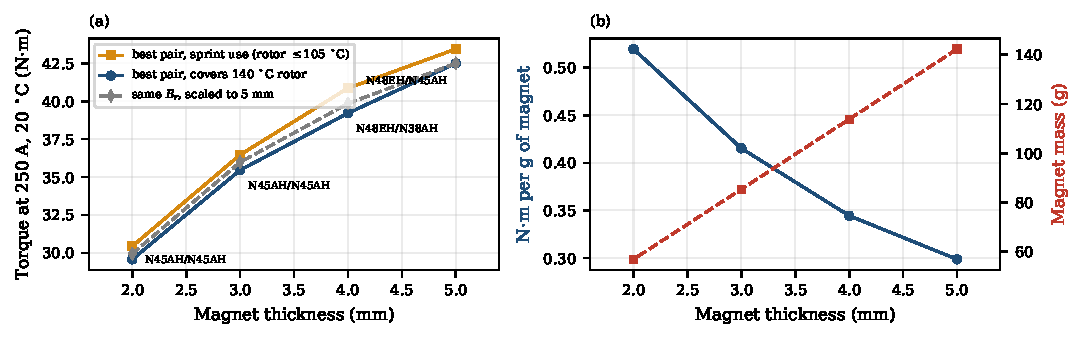
\includegraphics[width=\columnwidth]{thickness.pdf}
\caption{Magnet thickness. (a) Torque at \SI{250}{A} and \SI{20}{\celsius} for the best grade pair that covers a \SI{140}{\celsius} rotor, for the best pair for sprint use only, and for fixed $B_r$ (direct FEA, scaled to the 5-mm point). (b) Torque per gram of magnet and magnet mass.}
\label{fig:thick}
\end{figure}

\begin{table}[!t]
\caption{Magnet thickness: best grade pair and torque (ideal materials, \SI{250}{A})}\label{tab:thick}
\centering\footnotesize\setlength{\tabcolsep}{3.5pt}
\begin{tabular}{@{}cccccc@{}}
\toprule
$h_m$ & Pair (axial/side) & $T_{20}$ & $T_{100}$ & $T_\mathrm{mag,max}$ & Mass\\
(mm) & covers \SI{140}{\celsius} & (\Nm) & (\Nm) & nom./95\,\% (\si{\celsius}) & (g)\\
\midrule
5 & N48EH/N45AH & 42.5 & 38.8 & 145/137 & 142\\
4 & N48EH/N38AH & 39.2 & 35.9 & 142/136 & 114\\
3 & N45AH/N45AH & 35.5 & 32.3 & 149/142 & 85\\
2 & N45AH/N45AH & 29.6 & 26.9 & 143/137 & 57\\
\midrule
\multicolumn{6}{@{}l}{Sprint use only (rotor $\le$\SI{105}{\celsius}):}\\
5 & N50UH/N48EH & 43.4 & 39.6 & 117/-- & 142\\
4 & N50UH/N48EH & 40.9 & 37.2 & 111/-- & 114\\
3 & N48EH/N48EH & 36.5 & 33.2 & 121/-- & 85\\
2 & N48EH/N48EH & 30.4 & 27.6 & 115/-- & 57\\
\bottomrule
\end{tabular}
\end{table}


\Cref{fig:thick} and \cref{tab:thick} show the trade-off:
\begin{itemize}
\item \textbf{Torque falls by about \SI{3.5}{\Nm} per millimetre removed, and the fall accelerates below \SI{3}{mm}.} With the best pair for each thickness, \SI{4}{mm} gives \SI{-7.7}{\percent}, \SI{3}{mm} \SI{-16.6}{\percent} and \SI{2}{mm} \SI{-30}{\percent}.
\item \textbf{Torque per gram of magnet rises from 0.30 to \SI{0.52}{\Nm/g}.} This is why thin magnets are common where magnet cost or mass dominates.
\item \textbf{Thin magnets still need high-coercivity grades here.} In this machine the stator's reverse field at \SI{250}{A} is the design driver. Thinner magnets have a lower permeance coefficient, so they still need EH/AH grades to cover a hot rotor. The higher-$B_r$ grades do not become usable as the magnets get thinner.
\end{itemize}
Many published axial-flux motors with thin magnets are double-rotor or coreless, or run at lower electric loading, where this reverse field is weaker.

With the build and load factors of \cref{sec:realistic} (0.87) and the 6.6:1 reduction ($\eta=0.95$), the output torque at a \SI{100}{\celsius} rotor is about 213, 197, 177 and \SI{147}{\Nm} for 5, 4, 3 and \SI{2}{mm}. \SI{2}{mm} misses the \SI{180}{\Nm} target, and \SI{3}{mm} only meets it when the rotor is cool. \SI{4}{mm} is a reasonable trade if rotor inertia matters: it saves \SI{28}{g} and \SI{20}{\percent} of the magnet inertia for \SI{8}{\percent} torque. Otherwise \SI{5}{mm} remains the choice for maximum torque.
